\documentclass[11  pt]{exam} 
\usepackage[lmargin=1in,rmargin=1.75in,bmargin=1in,tmargin=1in]{geometry}  


% For hyperlinking everything
\usepackage{hyperref}
\hypersetup{
	colorlinks=true, %set true if you want colored links
	linktoc=all,     %set to all if you want both sections and subsections linked
	linkcolor=blue,  %choose some color if you want links to stand out
}


\usepackage[latin1]{inputenc}
\usepackage{amsmath}
\usepackage{mathrsfs}  
\usepackage{amsfonts}
\usepackage{amssymb}
\usepackage{graphicx}
\usepackage{subfig}
\usepackage{caption}
\usepackage{algorithm}
%\usepackage{algcompatible}
%\usepackage{algorithmicx}
\usepackage{algpseudocode}

\usepackage{titlesec}
\titleformat{\section}{\fontfamily{lmss}\fontsize{14}{15}\bfseries}{\thesection}{1em}{}
\titleformat{\subsection}{\fontfamily{lmss}\fontsize{12}{15}\bfseries}{\thesubsection}{1em}{}




\usepackage{amsthm}

\newtheoremstyle{noit}
{10pt}% <Space above>
{10pt}% <Space below>
{}% <Body font>
{}% <Indent amount>
{\bfseries}% <Theorem head font>
{.}% <Punctuation after theorem head>
{.5em}% <Space after theorem headi>
{}% <Theorem head spec (can be left empty, meaning `normal')>

\newtheoremstyle{example}
{10pt}% <Space above>
{10pt}% <Space below>
{}% <Body font>
{20pt}% <Indent amount>
{\bfseries}% <Theorem head font>
{.}% <Punctuation after theorem head>
{.5em}% <Space after theorem headi>
{}% <Theorem head spec (can be left empty, meaning `normal')>


\newtheoremstyle{indented}{20pt}{20pt}{\addtolength{\leftskip}{2.5em}}{}{\bfseries}{.}{.5em}{}


\newtheorem{theorem}{Theorem}
\numberwithin{theorem}{section}
\newtheorem{lemma}[theorem]{Lemma}
\newtheorem{corollary}[theorem]{Corollary}
\newtheorem{observation}{Observation}
%\numberwithin{observation}{section}
%\numberwithin{definition}{section}
\newtheorem{conjecture}{Conjecture}
\newtheorem{Qu}{Question}
\newcommand{\QU}{\begin{Qu}\normalfont}

\theoremstyle{noit}
\newtheorem{fact}{Fact}
\newtheorem{definition}{Definition}

\theoremstyle{indented}
\newtheorem{example}{Example}

\theoremstyle{indented}
\newtheorem{problem}{Problem}


%\newenvironment{proof}{\noindent{\bf Proof:} \hspace*{1em}}{
%    \hspace*{\fill} $\Box$ }
%\newenvironment{proof_of}[1]{\noindent {\bf Proof of #1:}
%    \hspace*{1em} }{\hspace*{\fill} $\Box$ }
%\newenvironment{proof_claim}{\begin{quotation} \noindent}{
%    \hspace*{\fill} $\diamond$ \end{quotation}}
\newcommand{\vs}[1]{\vspace{#1}}

\newcommand{\lecture}[2]{
 \noindent
\begin{center}
	\framebox{
		\vbox{
			\hbox to 5.78in { {\bf CSCE 411: Design and Analysis of Algorithms} \hfill  }
			\vspace{2mm}
			\hbox to 5.78in { {\Large \hfill Lecture #1\hfill} }
			\vspace{2mm}
			\hbox to 5.78in { {\it Date: #2 \hfill Lecturer: Nate Veldt} }
		}
	}
\end{center}
\vspace*{4mm}
}


\newcommand{\hw}[2]{
	\noindent
	\begin{center}
		\framebox{
			\vbox{
				\hbox to 5.78in { {\bf CSCE 411: Design and Analysis of Algorithms} \hfill  }
				\vspace{2mm}
				\hbox to 5.78in { {\Large \hfill Homework #1\hfill} }
				\vspace{2mm}
				\hbox to 5.78in { {\it Due date: #2 \hfil} }
			}
		}
	\end{center}
	\vspace*{4mm}
}



\newcommand{\under}[1]{\underline{\hspace{#1}}}
\setlength{\parindent}{0em}

%\usepackage[tagged]{accessibility}

% Graph terms
\newcommand{\vol}{\textbf{vol}}
\newcommand{\cut}{\textbf{cut}}


% Matrices
\newcommand{\mA}{\textbf{A}}
\newcommand{\mB}{\textbf{B}}

% vectors
\newcommand{\ve}{\textbf{e}}
\newcommand{\vx}{\textbf{x}}


% Other
\newcommand{\calN}{\mathcal{N}}

\usepackage{mathtools}
\DeclarePairedDelimiter\ceil{\lceil}{\rceil}
\DeclarePairedDelimiter\floor{\lfloor}{\rfloor}


\newcommand*{\aitem}{ \item[{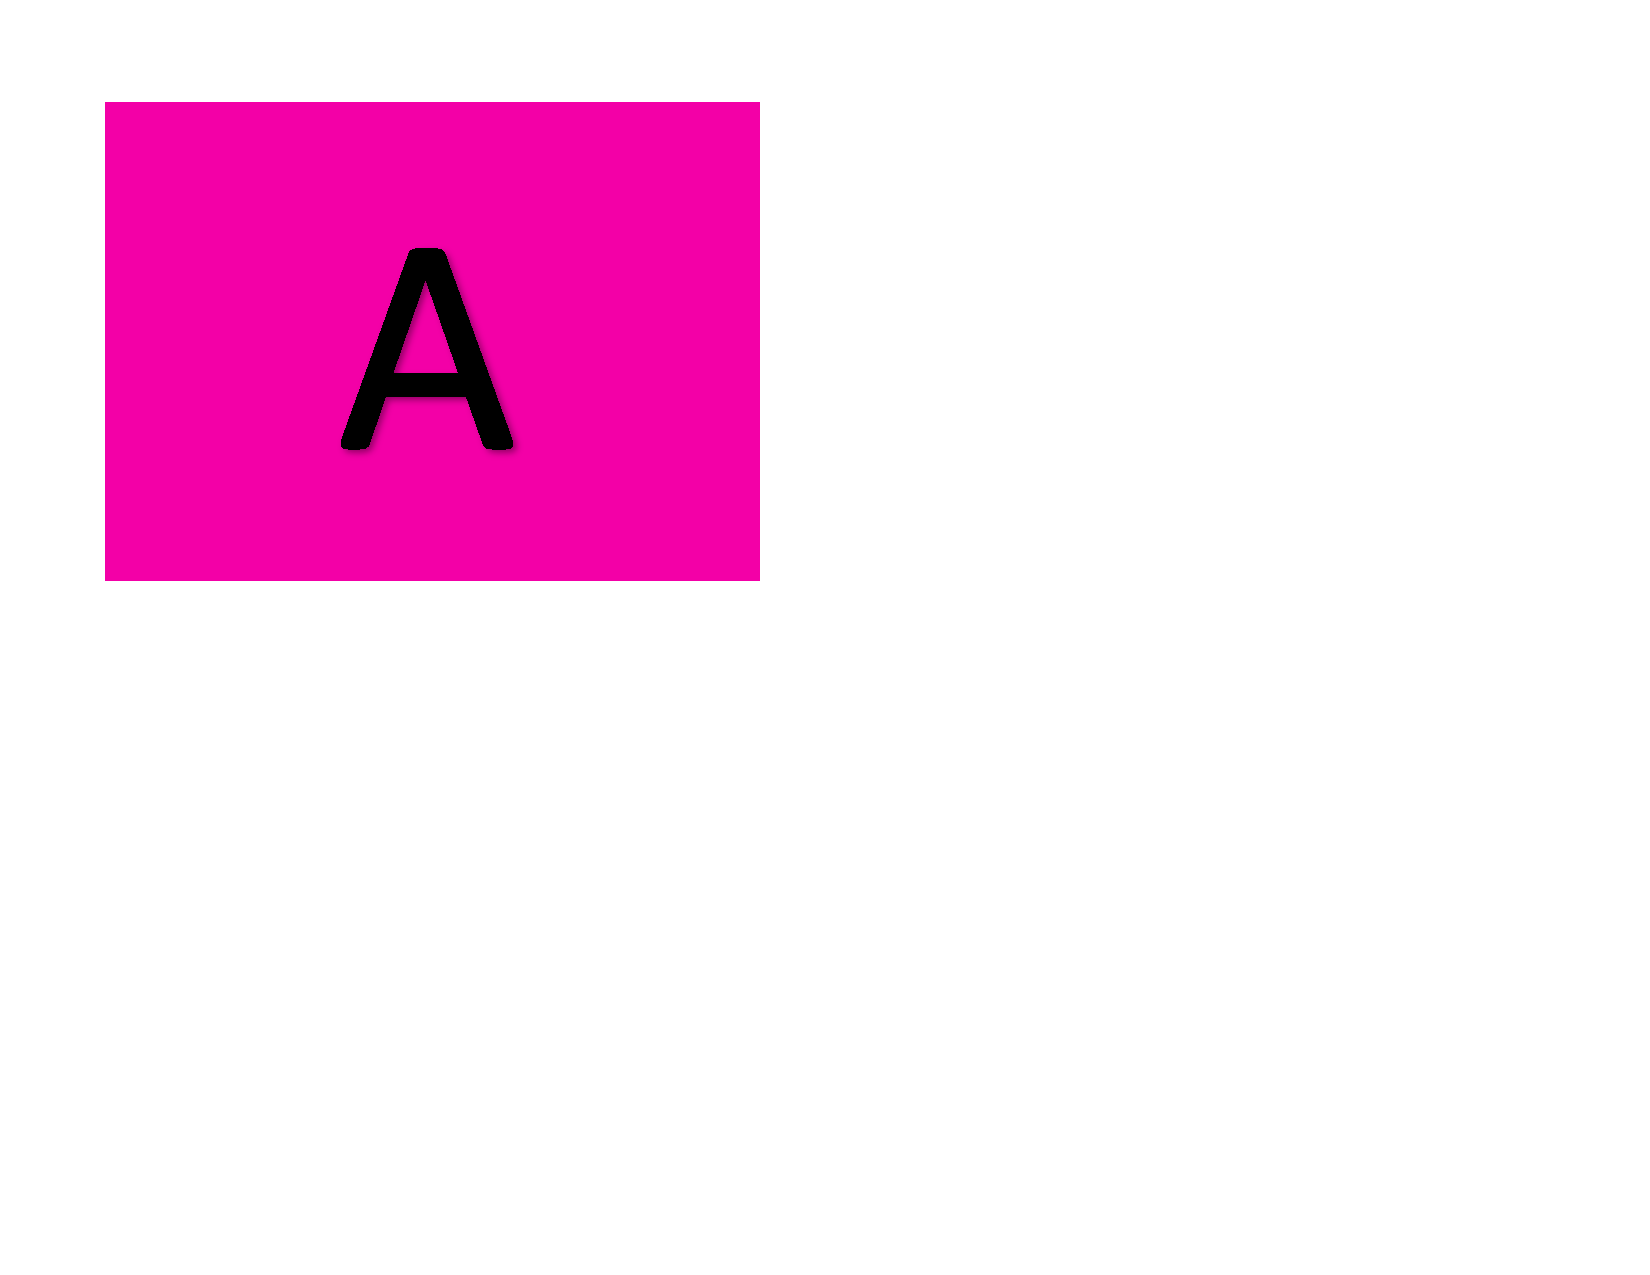
\includegraphics[width=0.8cm,height=0.5cm]{../../Lectures/figures/A}} ]  }
\newcommand*{\bitem}{ \item[{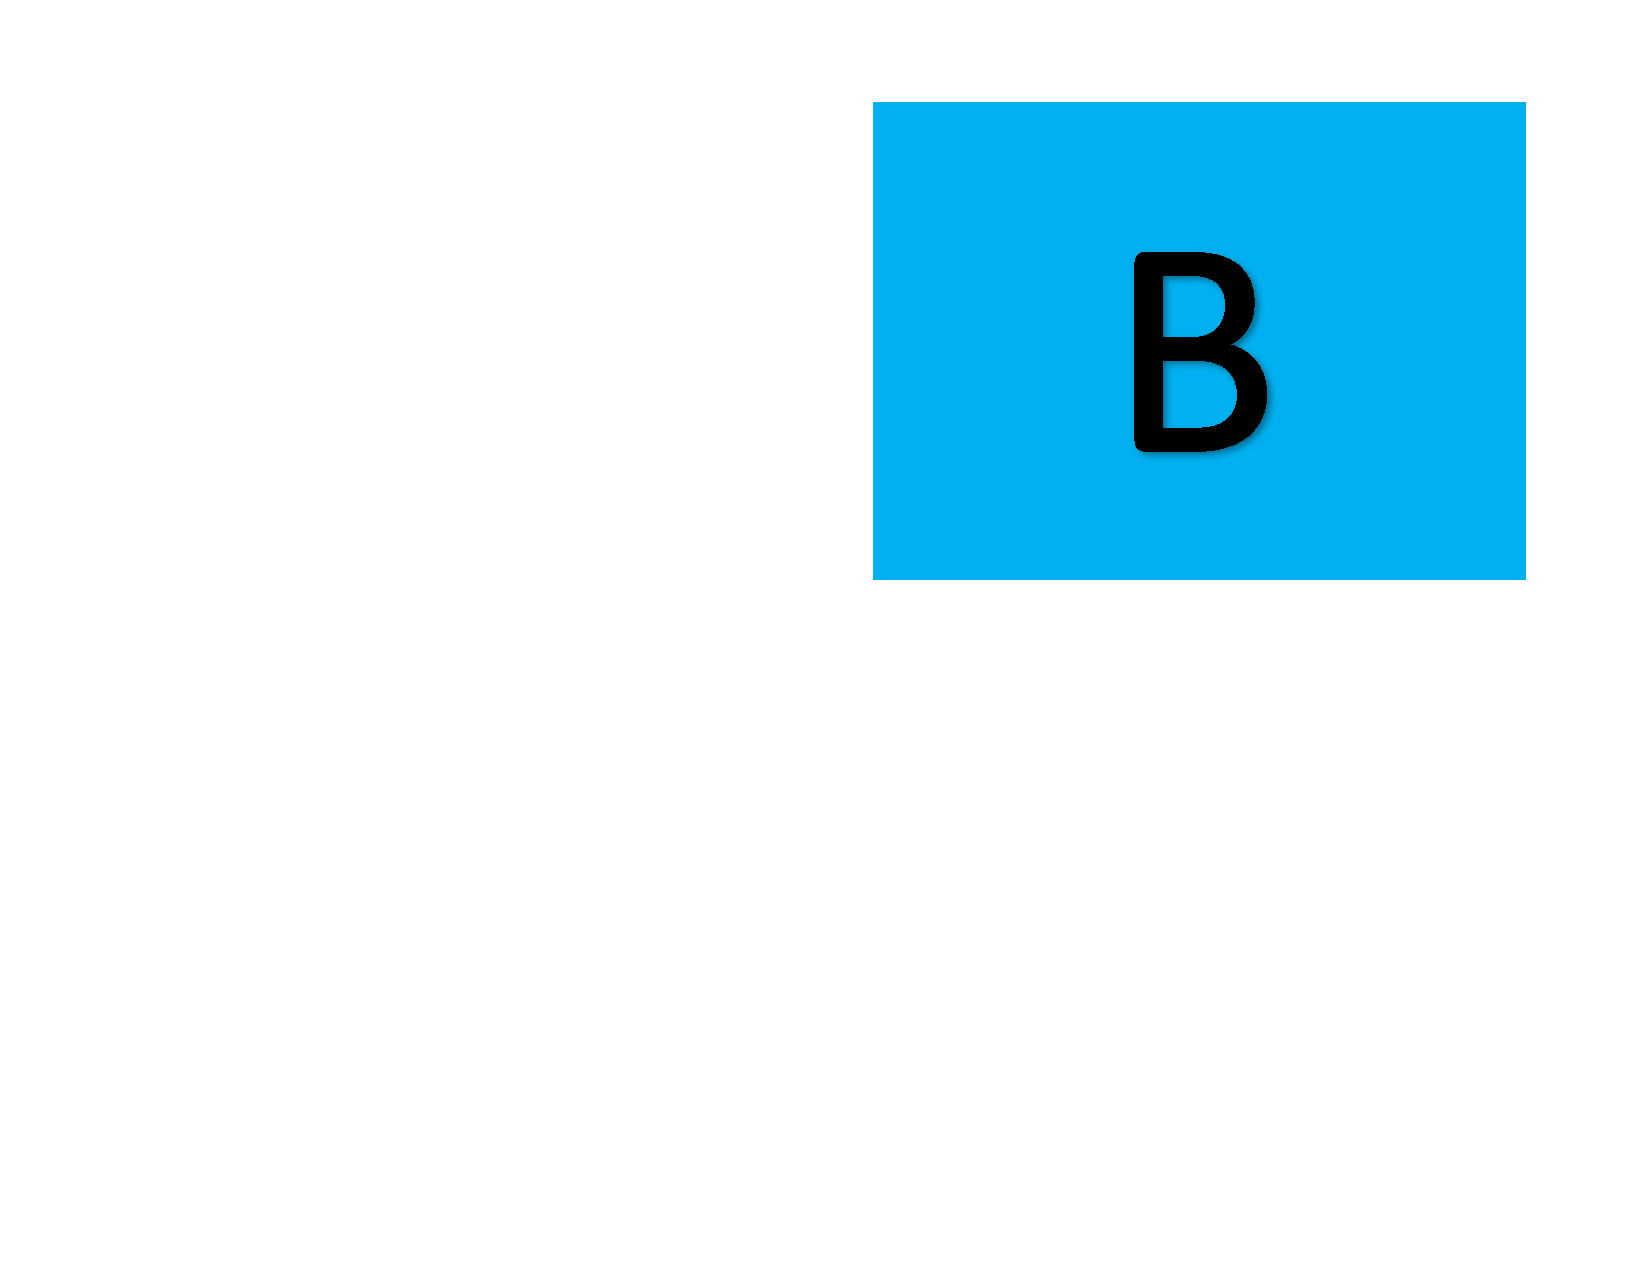
\includegraphics[width=0.8cm,height=0.5cm]{../../Lectures/figures/B}} ]  }
\newcommand*{\citem}{ \item[{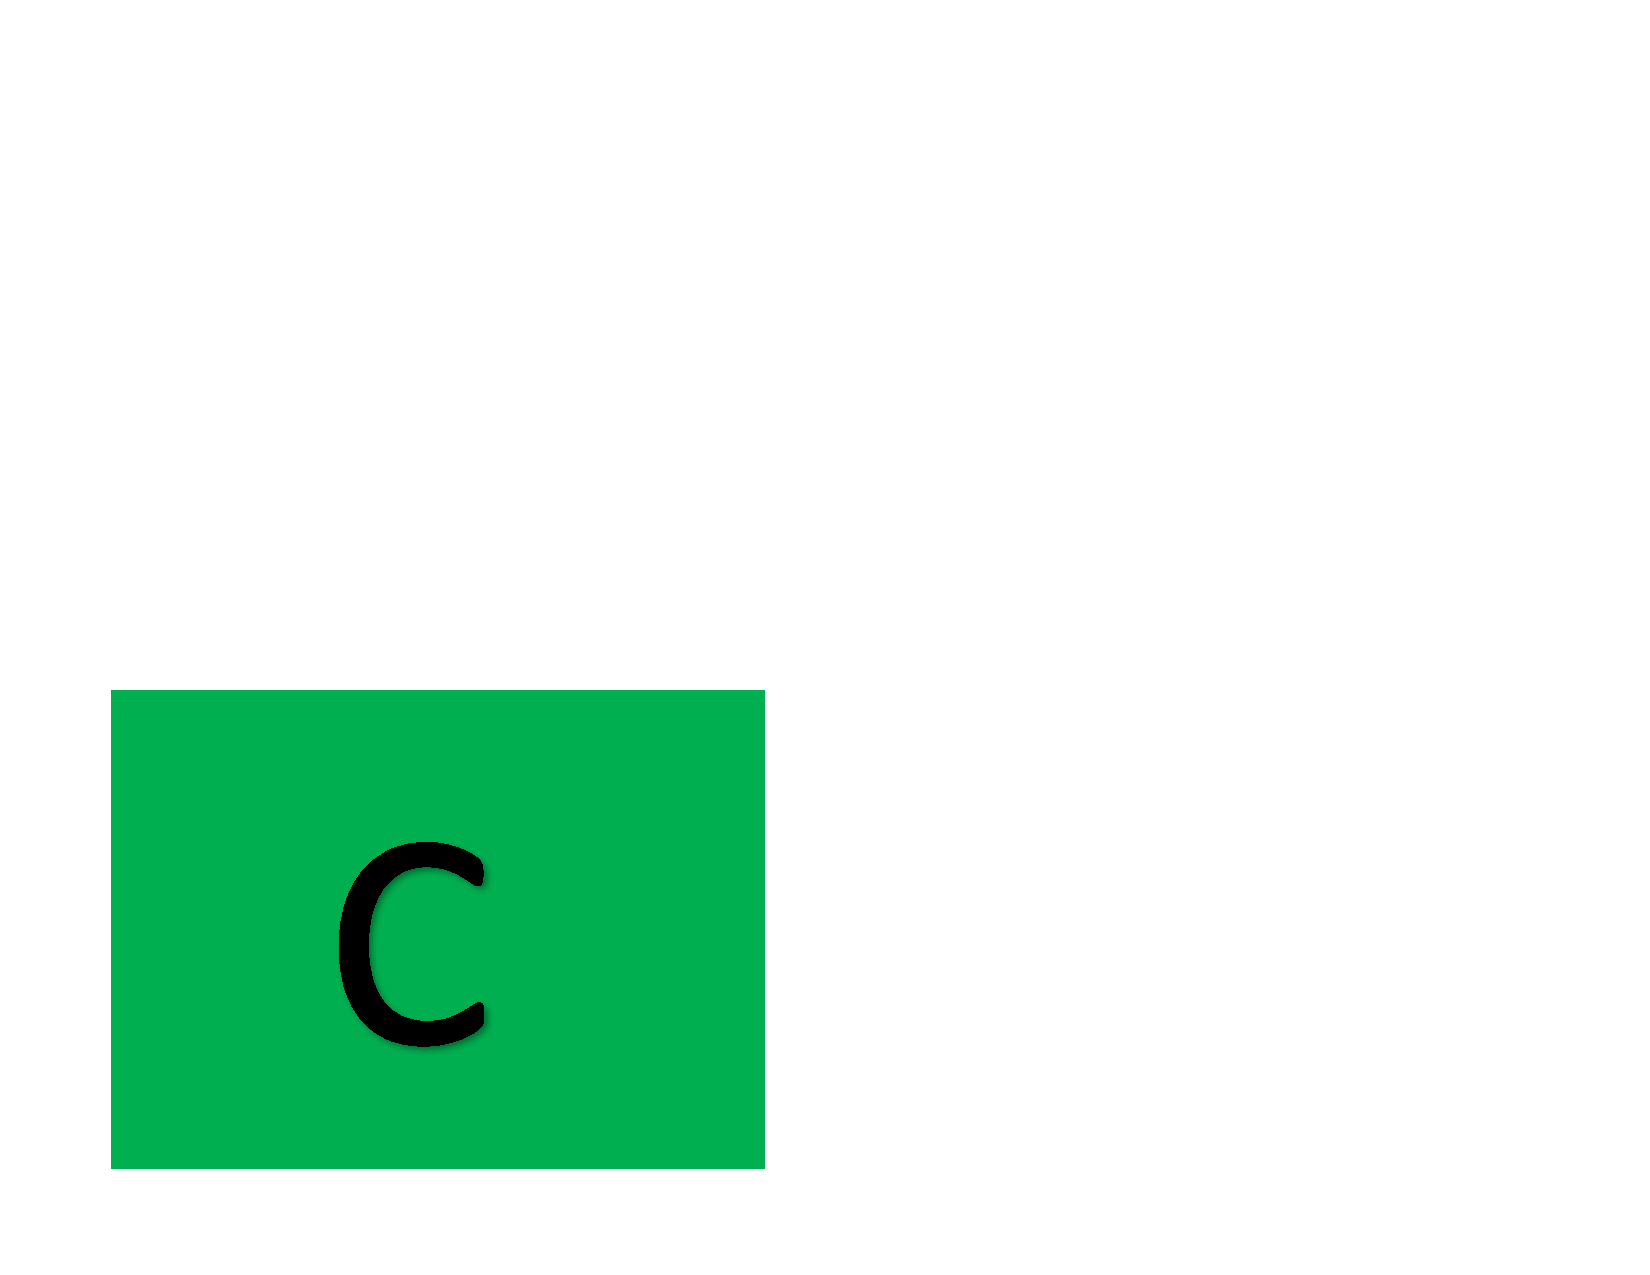
\includegraphics[width=0.8cm,height=0.5cm]{../../Lectures/figures/C}} ]  }
\newcommand*{\ditem}{ \item[{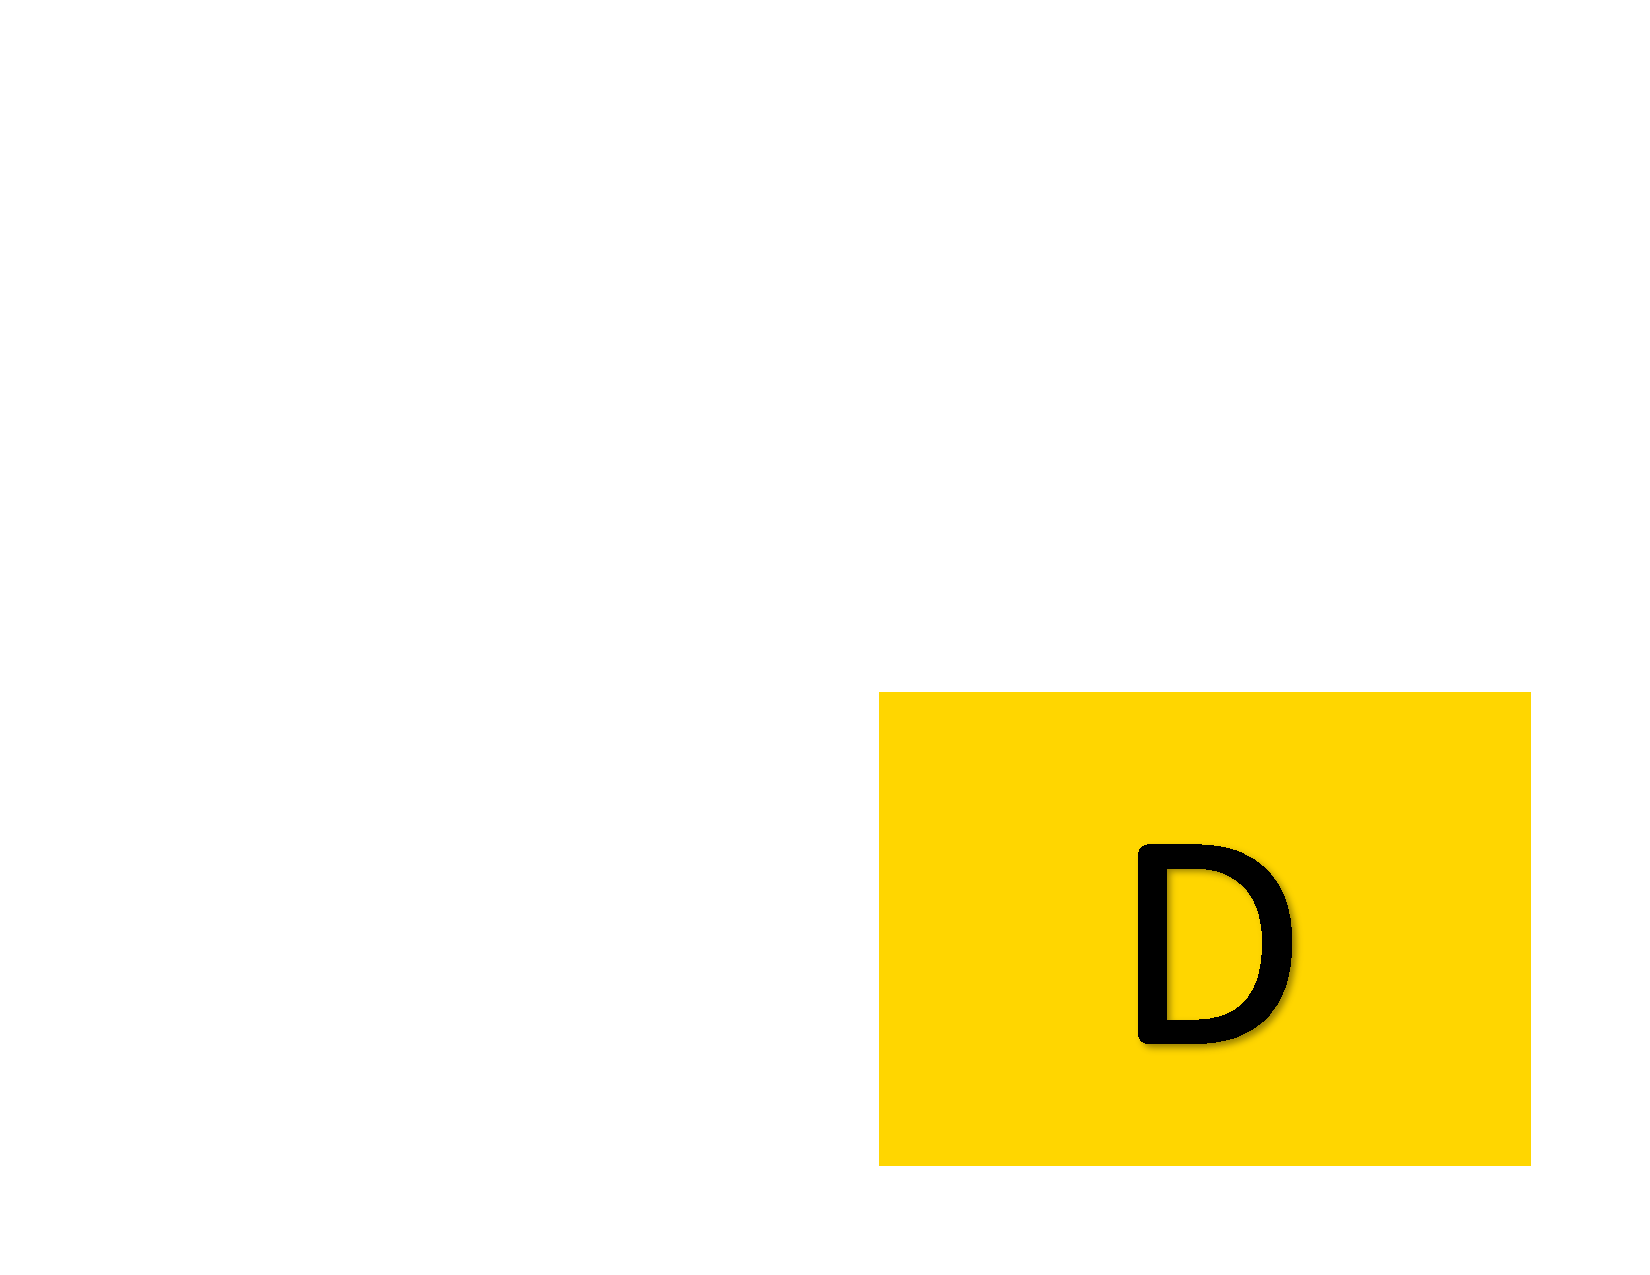
\includegraphics[width=0.8cm,height=0.5cm]{../../Lectures/figures/D}} ]  }
\newcommand*{\eitem}{ \item[{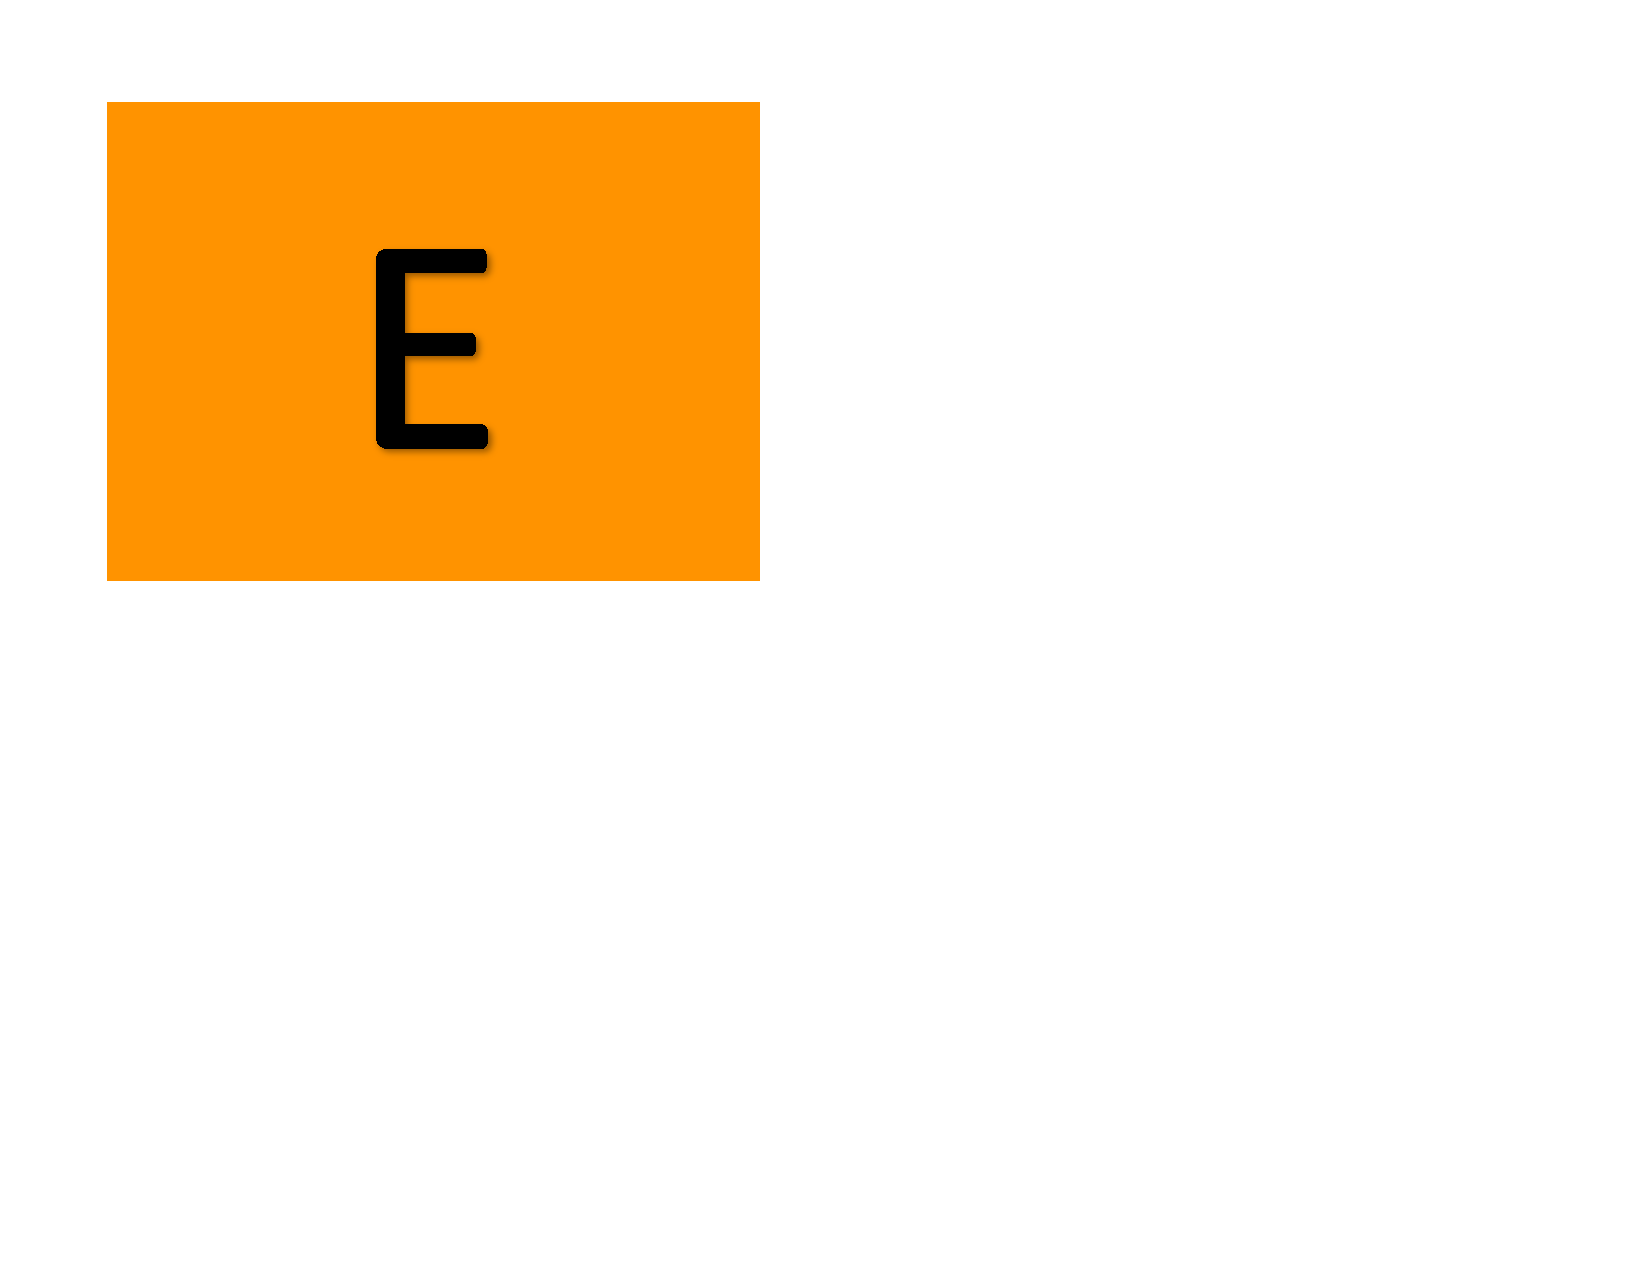
\includegraphics[width=0.8cm,height=0.5cm]{../../Lectures/figures/E}} ]  }
\newcommand*{\fitem}{ \item[{
\includegraphics[width=0.8cm,height=0.5cm]{../../Lectures/figures/F}} ]  }


\newcommand{\hide}[1]{\underline{\phantom{#1 #1}}}

\usepackage{setspace}

\onehalfspacing



\begin{document}
	
	\lecture{14: Single-Source Shortest Path}{March 6}
	
	
	\paragraph{Course Logistics}
	\begin{itemize}
		\item Reading from Chapter 24 this week, especially sections 24.1, and 24.3
		\item Homework 5 due Friday (tomorrow)
	\end{itemize}
	
	\section{The Single-Source (weighted) Shortest Paths Problem}
	Consider a directed and weighted graph $G = (V,E, w)$, where $w \colon E \rightarrow \mathbb{R}$ maps edges to weights.\\
	
	Given a path $p = \{v_0, v_1, \hdots , v_k\}$ from $i = v_0$ to $j = v_k$, 
	
	\vs{2.5cm}
	
	
	the weight of the path $p$ is given by: 
\vs{3cm}
	
	Let $\mathcal{P}_{ij}$ be the set of paths from nodes $i$ to $j$. The \emph{shortest path weight} from $i$ to $j$ is:
	\begin{equation*}
		\delta(i,j) = \begin{cases}
		 \\  \\%	\min_{p} \\%w(p) & \text{if there is a path $p$ from $i$ to $j$} \\ \\
			\infty & % \text{otherwise}
		\end{cases}
	\end{equation*}
	A \hide{shortest path} from $u$ to $v$ is a path $p$ such that $\delta(u,v) = w(p)$. \\
	
	\paragraph{Definition} Given a \emph{source} node $s \in V$, the single-source shortest paths problem (SSSP) seeks to find the shortest path weight $\delta(s,u)$ for every $u \in V$.
	
	\newpage
	
	
	\subsection{Shortest Path Properties}
	
	\paragraph{Triangle Inequality}
	For any set of three nodes $s$, $u$, and $v$,
	\begin{equation*}
		\delta(s,u) \leq \delta(s,v) + \delta(v,u) \\
	\end{equation*}
	
	\paragraph{Optimal Substructure}
	\begin{lemma} If $p = \{v_0, v_1, \hdots , v_k\}$ is a shortest path from $v_0$ to $v_k$, then all of its subpaths \hide{are shortest paths as well. }
	\end{lemma}
	
	\vs{5cm}
	
	\paragraph{Cycles and shortest paths}
	\begin{lemma}: If $G = (V,E,w)$ has no negative edges, then %no shortest path contains a cycle.
	\end{lemma}
	\vs{2cm}
	
	
	\newpage
	
	\subsection{Negative edges}
	\begin{Qu}
		Assume $G = (V,E, w)$ contains negative edges, and that it is strongly connected. If $G$ contains a cycle where the sum of edge weights is negative, which of the following is true?
		\begin{itemize}
			\aitem The shortest path weight between every pair of nodes will be a finite negative number
			\bitem The shortest path weight between some (but not necessarily all nodes) will be a finite negative number
			\citem The shortest path weight can be $-\infty$ for some pairs of nodes, but not necessarily all pairs of nodes
			\ditem The shortest path weight will be $-\infty$ between all pairs
		\end{itemize}
	\end{Qu}
	\vs{5cm}
	
	\newpage
	\subsection{SSSP Algorithm Basics}
	Let $s$ denote the starting node of an SSSP problem. In shortest path algorithms, we maintain two attributes for each $v \in V$: \\
	
	
	\begin{tabular}{| l | p{4.5cm} | p{4.5cm} | p{4.5cm} |}
		\hline
		\textbf{Attribute} & \textbf{Explanation} & \textbf{Initialization} & \textbf{Invariant} \\
		\hline
		$u.d$ & \phantom{the best guess for the distance from $s$ to $u$} \newline &  \phantom{$s.d = 0$;} \newline \phantom{$u.d = \infty$ for $u \neq s$} & \phantom{We will always maintain:  $u.d \geq \delta(s,d)$} \\
		\hline
		$u.\pi$ \newline &  \phantom{the predecessor of $u$ in a path from $s$ to $u$ dfasdfsfd}\newline \phantom{the predecessor of $u$ in a path from $s$ to $u$ dfasdfsfd} &  & \\
		\hline
	\end{tabular}
	
	\vs{2cm}
	
	Given values for these attributes, we can construct a \emph{predecessor} graph:
	\begin{itemize}
		\item $V_\pi = \{ v \in V \colon v.\pi \neq \text{NIL}\} \cup \{s\}$ \\\
		\item $E_\pi = \{(v.\pi, v) \colon v \in V_\pi - \{s\}\}$
	\end{itemize}
	
	
	If $v.d = \delta(s,v)$ and $v.\pi$ gives the predecessor of $v$ in a shortest path from $s$ to $v$, then $G_\pi = (V_\pi, E_\pi)$ is called a \hide{shortest path tree}.
	
	\vs{3cm}
	
	
	
	\newpage
	
	\subsection{Relaxation and Generic Algorithm}
	The key idea behind shortest path algorithms is to successively ``relax'' edges.
	\begin{algorithm}
		\textsc{Relax}($u,v,w$)
		\begin{algorithmic}
			\If{$v.d > u.d + w(u,v)$}
			\State 
			\State
			\State
			\State
			\EndIf
		\end{algorithmic}
	\end{algorithm}
	
	\vs{5cm}
	\begin{algorithm}
		\textsc{GenericSSSP}($G,w,s$)
		\begin{algorithmic}
			\State \textsc{Initialize-SSSP}$(G,w,s)$
			\While{There is some edge $(u,v)$ with $v.d > u.d + w(u,v)$}
			\State 
			\State
			\State
			\State
			\EndWhile
		\end{algorithmic}
	\end{algorithm}
	
	\newpage
	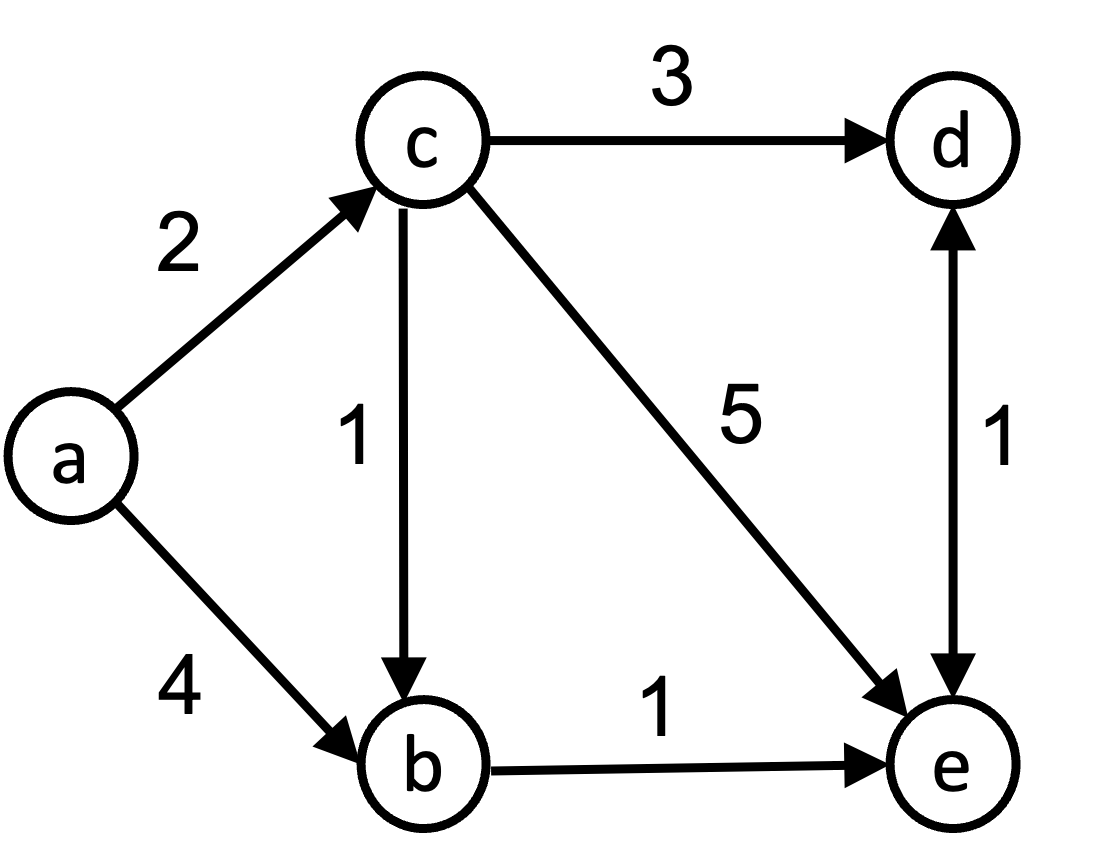
\includegraphics[width = .45\linewidth]{small-graph-sssp.png}
	
	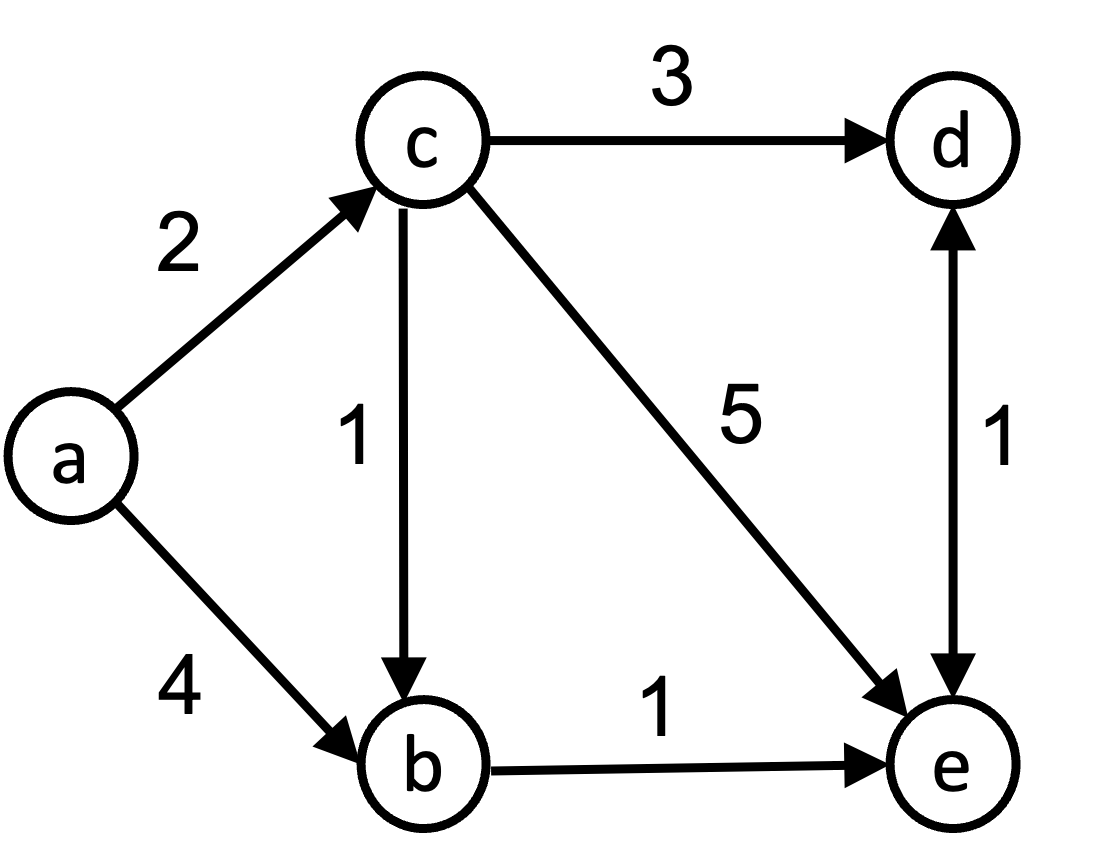
\includegraphics[width = .45\linewidth]{small-graph-sssp.png}
	
	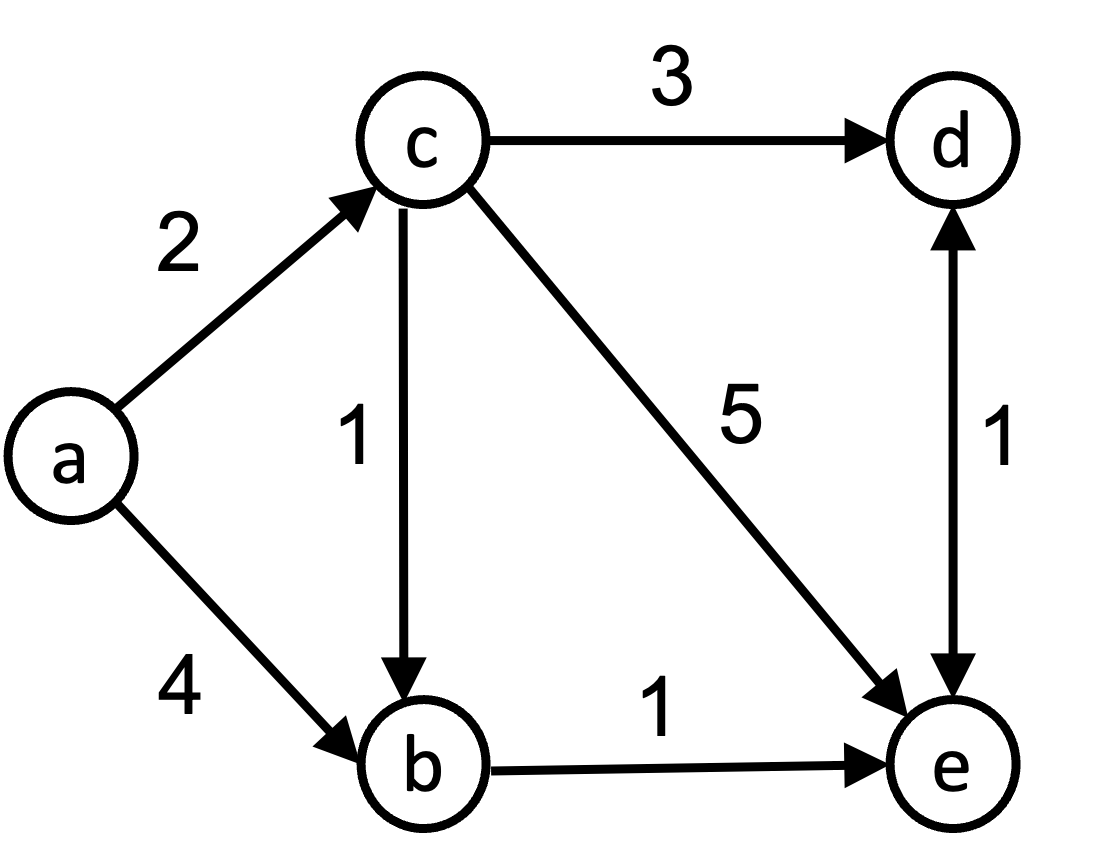
\includegraphics[width = .45\linewidth]{small-graph-sssp.png}
	
	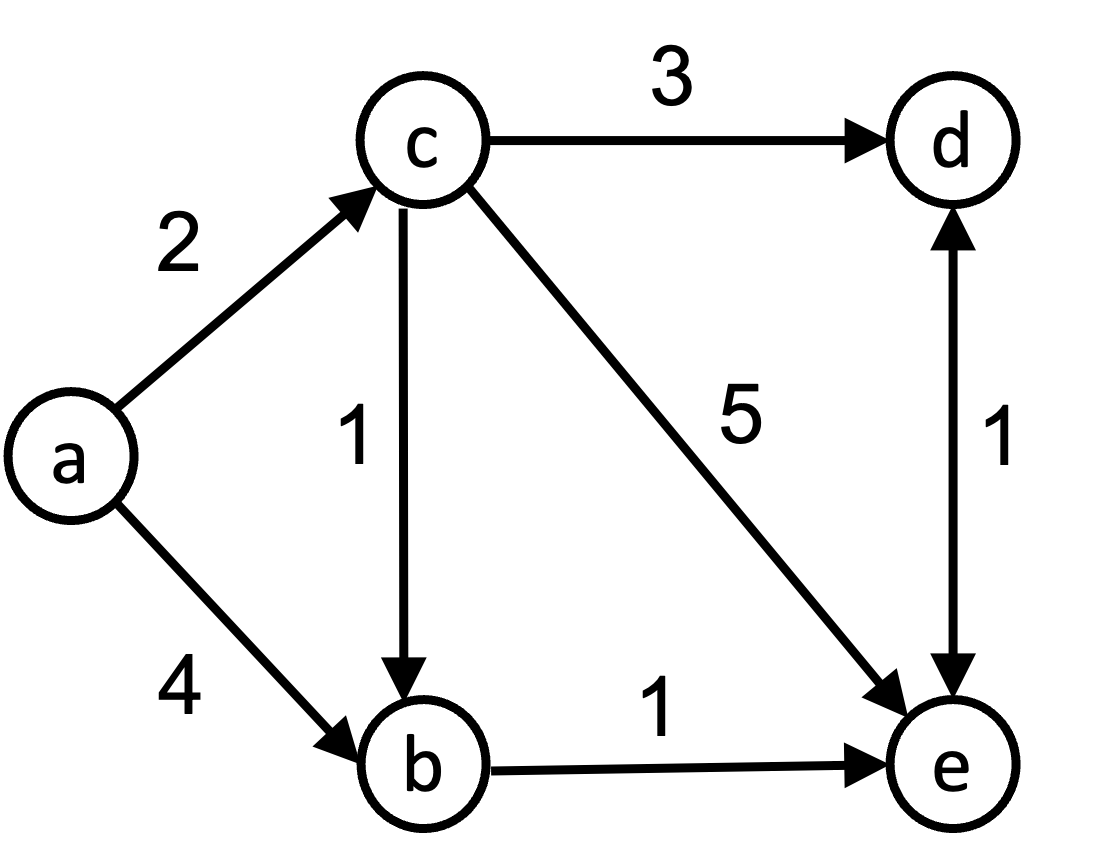
\includegraphics[width = .45\linewidth]{small-graph-sssp.png}
	
	\newpage 
	
	\section{The Bellman Ford Algorithm}
	
	Let's do a quick recap of what we have learned so far about the SSSP problem.

	\paragraph{Cycles} Let $p$ be a cycle in a directed graph.
	
	\begin{itemize}
		\item Case 1: $w(p) \geq 0$: then I can get rid of the cycle and I have a better path 
		\item Case 2: $w(p) < 0$: then all paths are of length $-\infty$ because we can traverse $p$ as many times as we want to decrease the path weight. 
	\end{itemize}
	
	If Case 2 is true, we would prefer to be aware of this, in which case we state that all shortest paths have weight $-\infty$ and we're done.
	
	Otherwise, we do not seek out paths with cycles when solving the SSSP problem.
	
	\paragraph{Relaxations and Generic Algorithm} 
	\begin{algorithm}
		\textsc{Relax}($u,v,w$)
		\begin{algorithmic}
			\If{$v.d > u.d + w(u,v)$}
			\State $v.d = u.d + w(u,v)$
			\State $v.\pi = u$
			\EndIf
		\end{algorithmic}
	\end{algorithm}
	\begin{algorithm}
		\textsc{GenericSSSP}($G,w,s$)
		\begin{algorithmic}
			\State \textsc{Initialize-SSSP}$(G,w,s)$
			\While{There is some edge $(u,v)$ with $v.d > u.d + w(u,v)$}
			\State \textsc{Relax}($u,v,w$)
			\EndWhile
		\end{algorithmic}
	\end{algorithm}
	
	Now we are ready to find a more concrete implementation of this approach, by answering the question:
	

	\newpage
	\subsection{Bellman-Ford Algorithm Pseudocode}
	
	\begin{algorithm}
		\textsc{Bellman-Ford}($G,w,s$)
		\begin{algorithmic}
			\For{$v \in V$}
			\State $v.d = \infty$
			\State $v.\pi = \text{NIL}$
			\EndFor
			\State $s.d = 0$
			\State 
			\For{$i = 1$ to $|V| - 1$}
			\For{$ (u,v) \in E$}
			\State $\textsc{Relax}(u,v,w)$
			\EndFor
			\EndFor
			\State 
			\For{$ (u,v) \in E$}
			\If{$v.d > u.d + w(u,v)$}
			\State Return ``the graph has a negative cycle"
			\EndIf
			\EndFor
			\State
			\State $V_\pi = \{ v \in V \colon v.\pi \neq \text{NIL}\} \cup \{s\}$
			\State $E_\pi = \{(v.\pi, v) \colon v \in V_\pi - \{s\}\}$
			\State Return $(V_\pi, E_\pi)$ and $\{v.d \colon v \in V\}$
		\end{algorithmic}
	\end{algorithm}
	
	\begin{Qu}
		What is the runtime complexity of running the \textsc{Bellman-Ford} Algorithms?
		\begin{itemize}
			\aitem $O(V + E)$
			\bitem $O(E \log V)$
			\citem $O(E + V \log V)$
			\ditem $O(EV)$
		\end{itemize}
	\end{Qu}
	
	\newpage
	
	\begin{algorithm}[t]
		\textsc{Bellman-Ford}($G,w,s$)
		\begin{algorithmic}
			\State \textsc{InitializeSSSP}($G,w,s)$
			\For{$i = 1$ to $|V| - 1$}
			\For{$ (u,v) \in E$}
			\State $\textsc{Relax}(u,v,w)$
			\EndFor
			\EndFor
			\State Return $\{v.d\}$
		\end{algorithmic}
	\end{algorithm}
	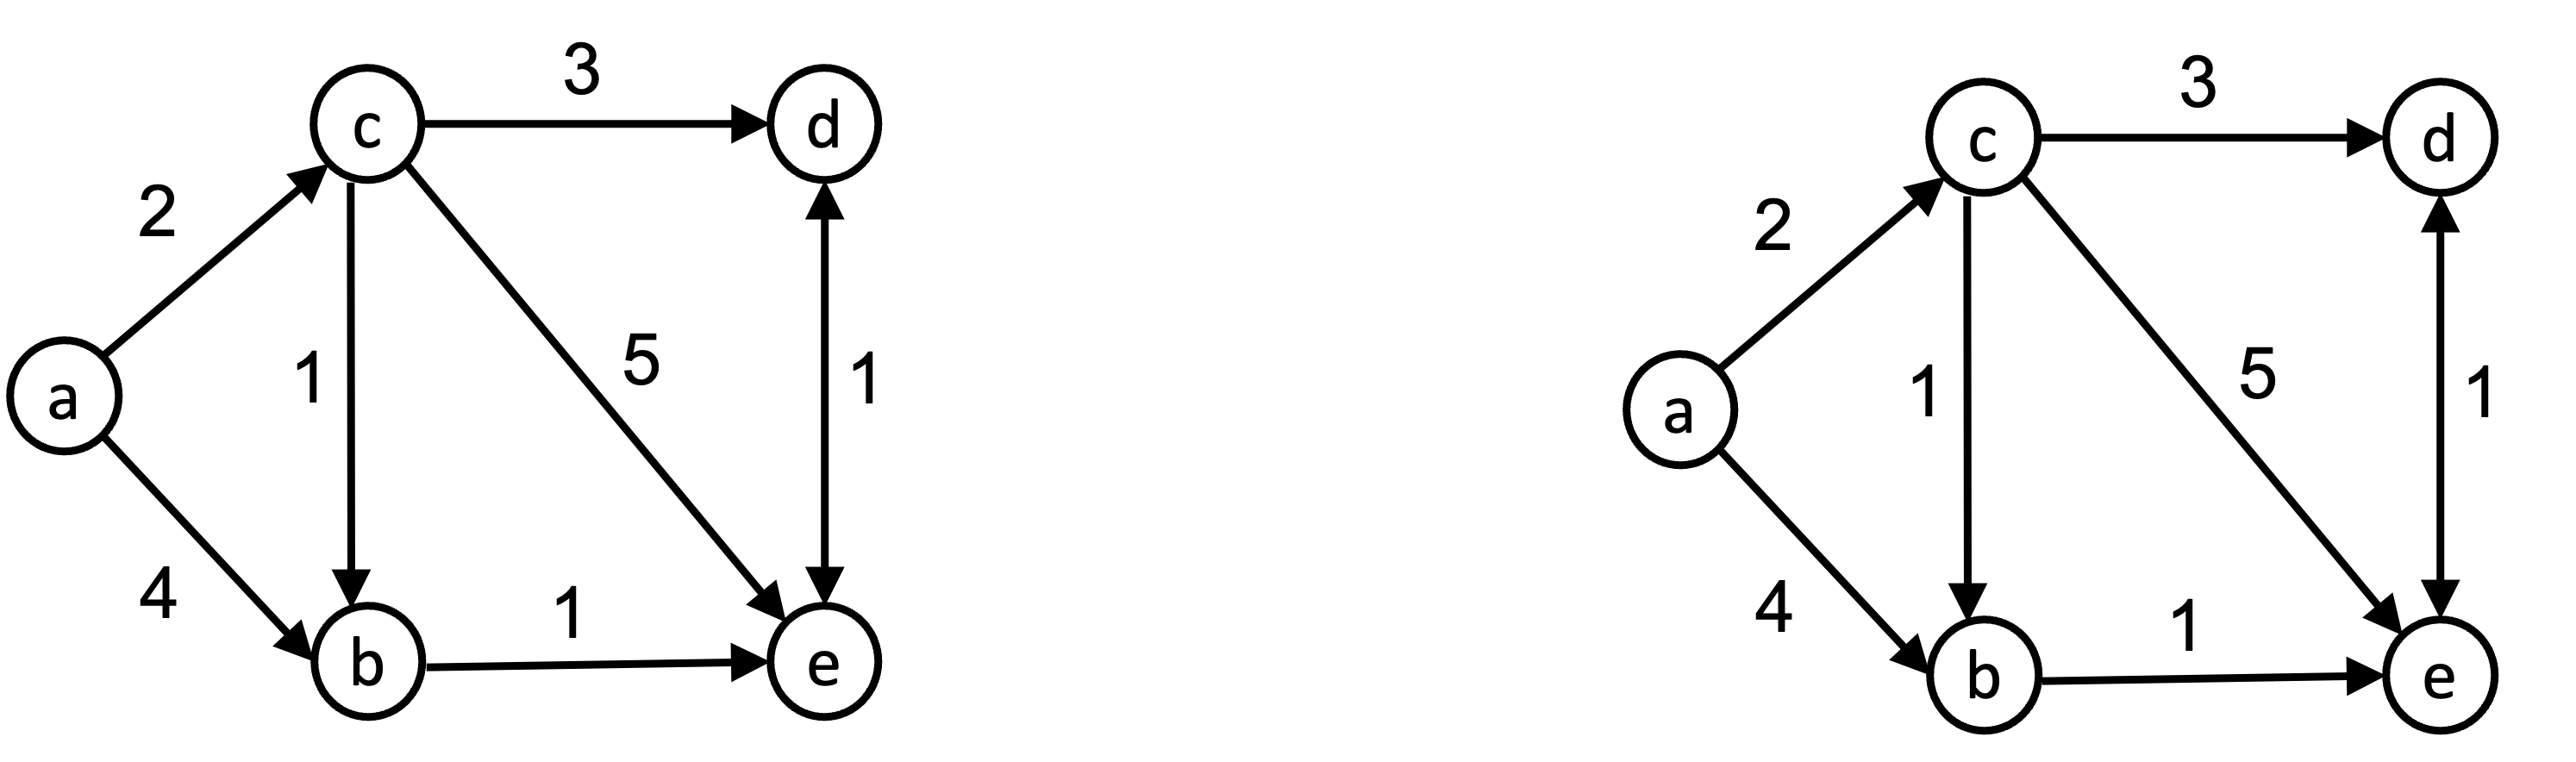
\includegraphics[width = \linewidth]{twographs.png}
	
	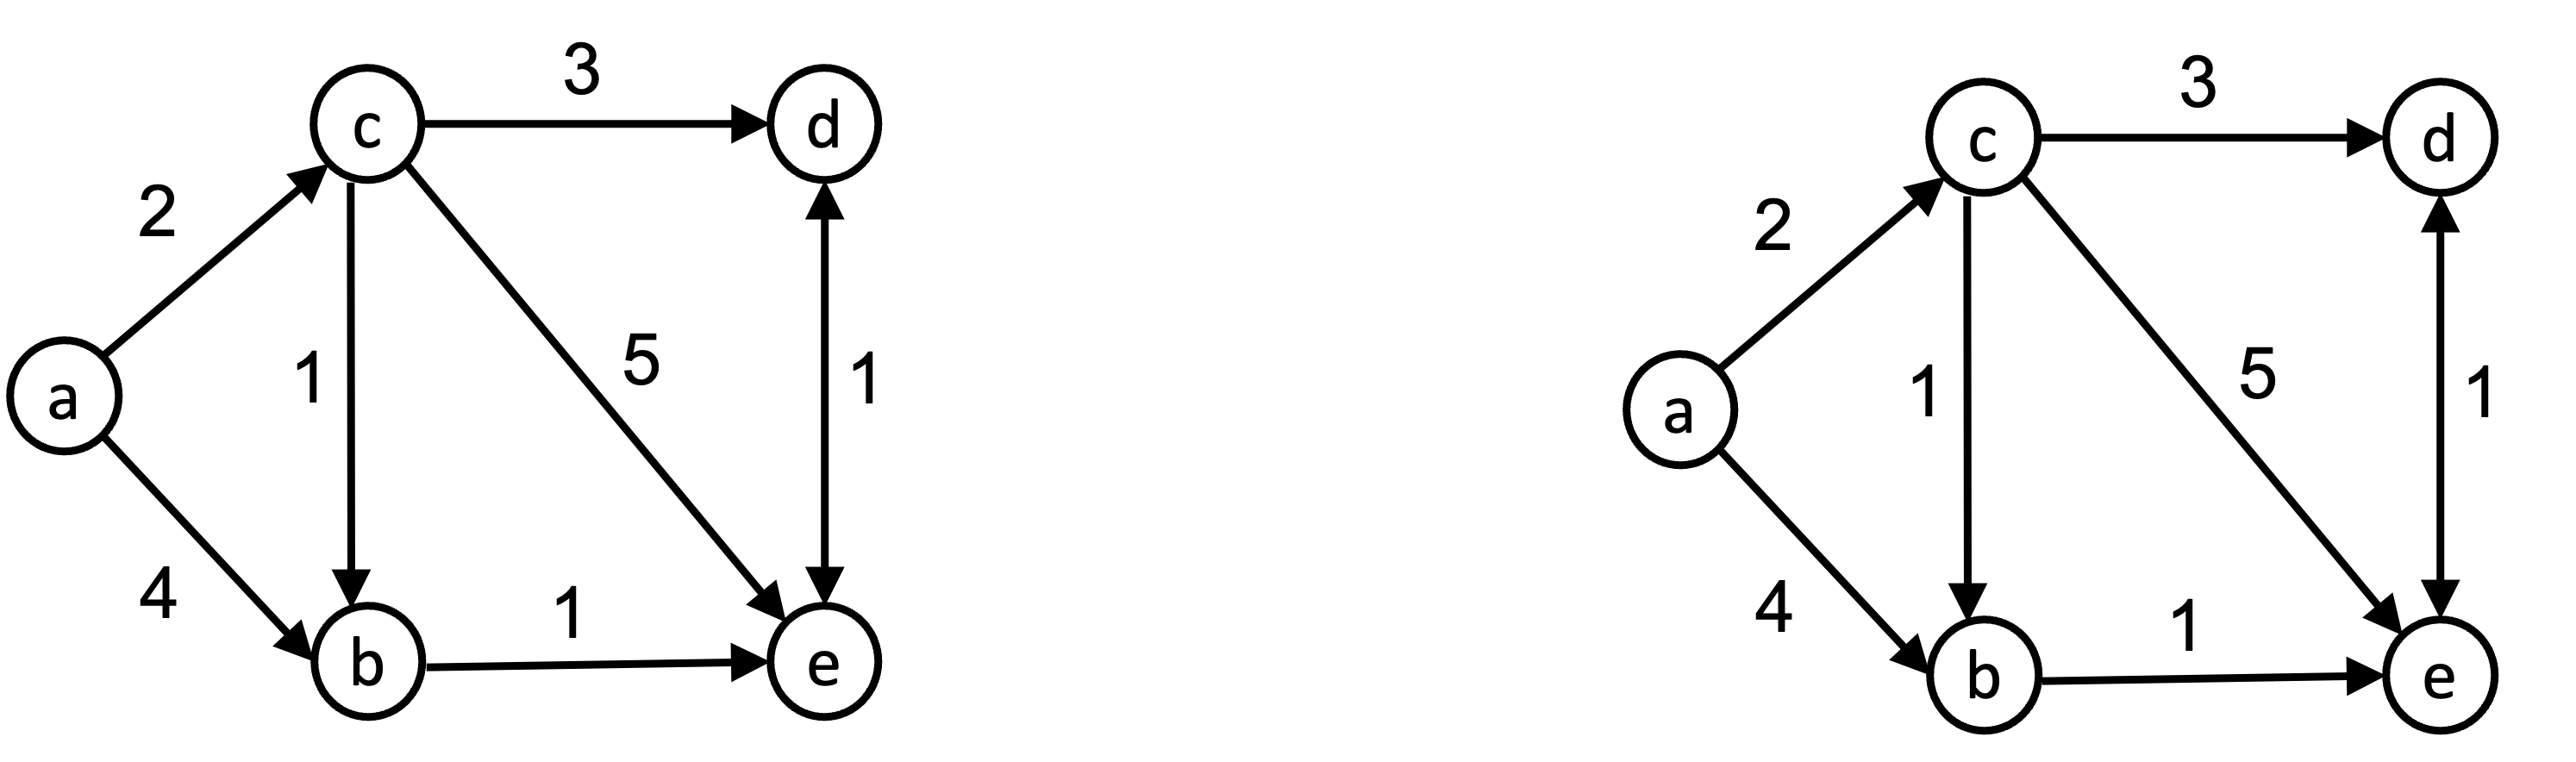
\includegraphics[width = \linewidth]{twographs.png}
	
	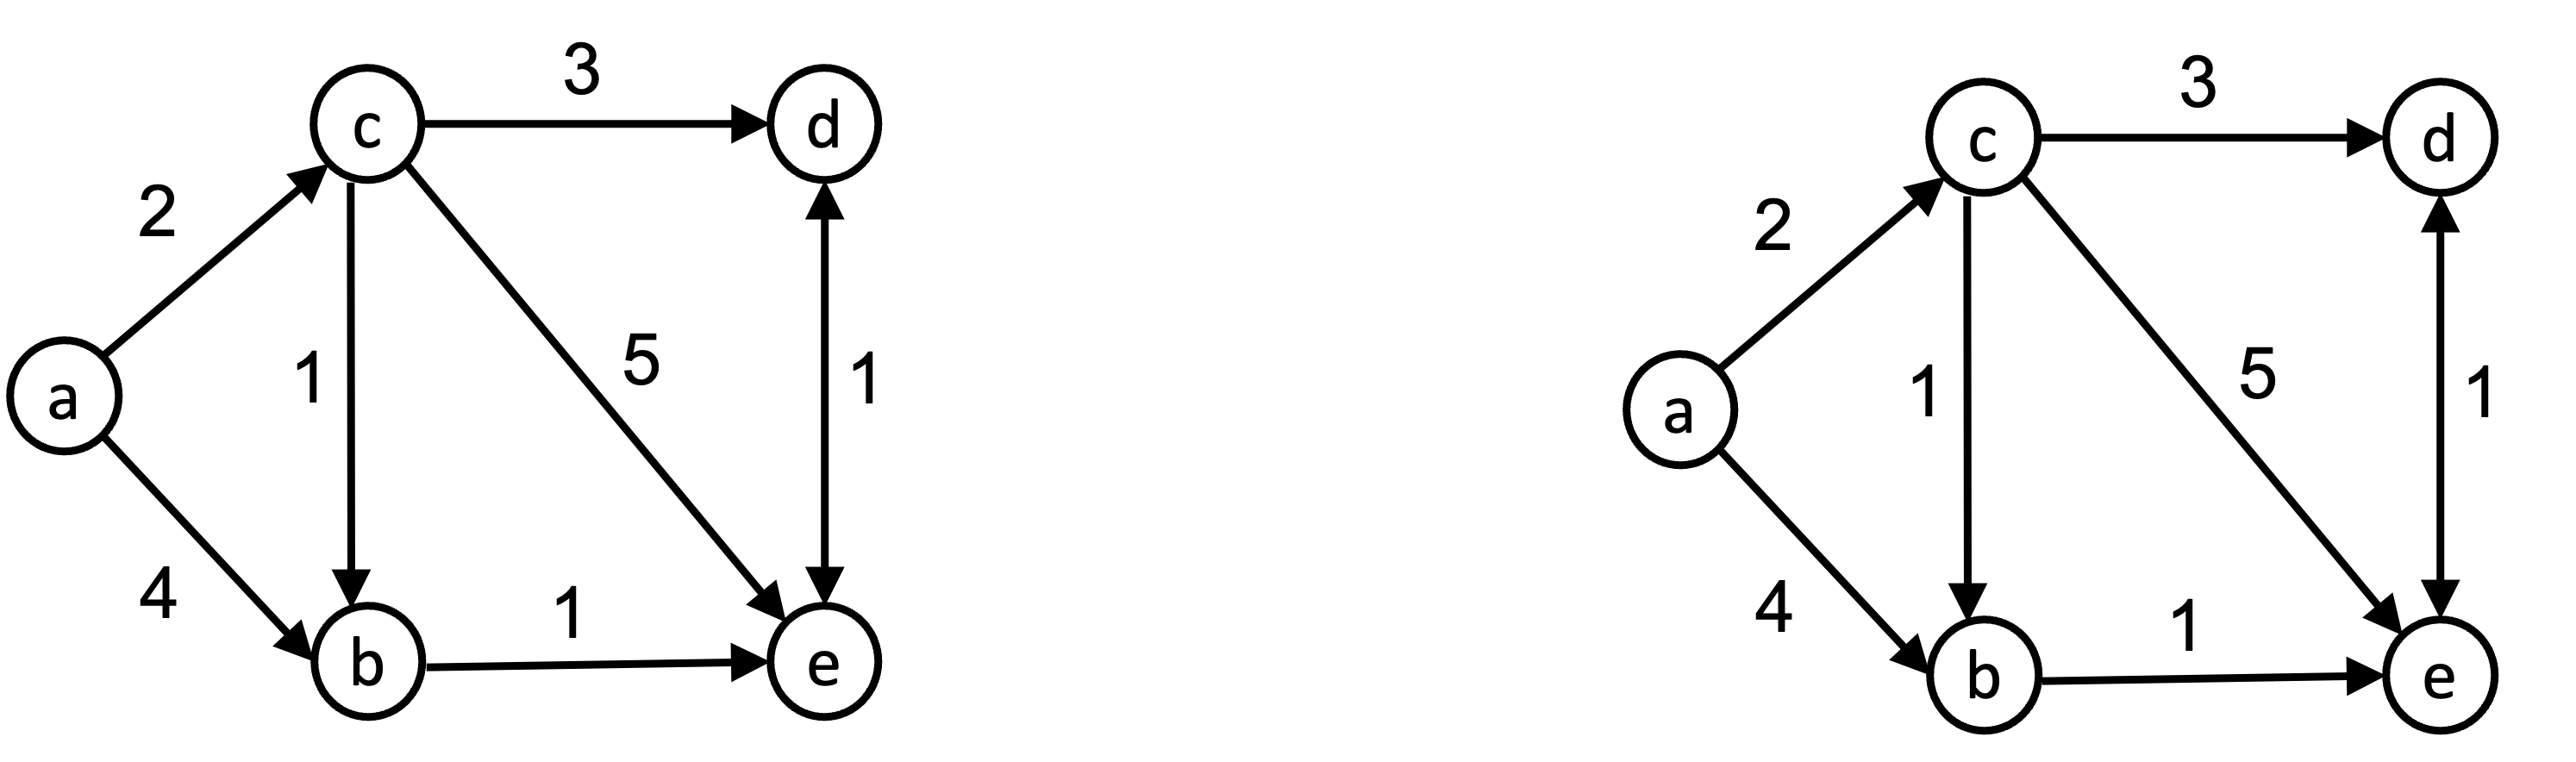
\includegraphics[width = \linewidth]{twographs.png}
	
	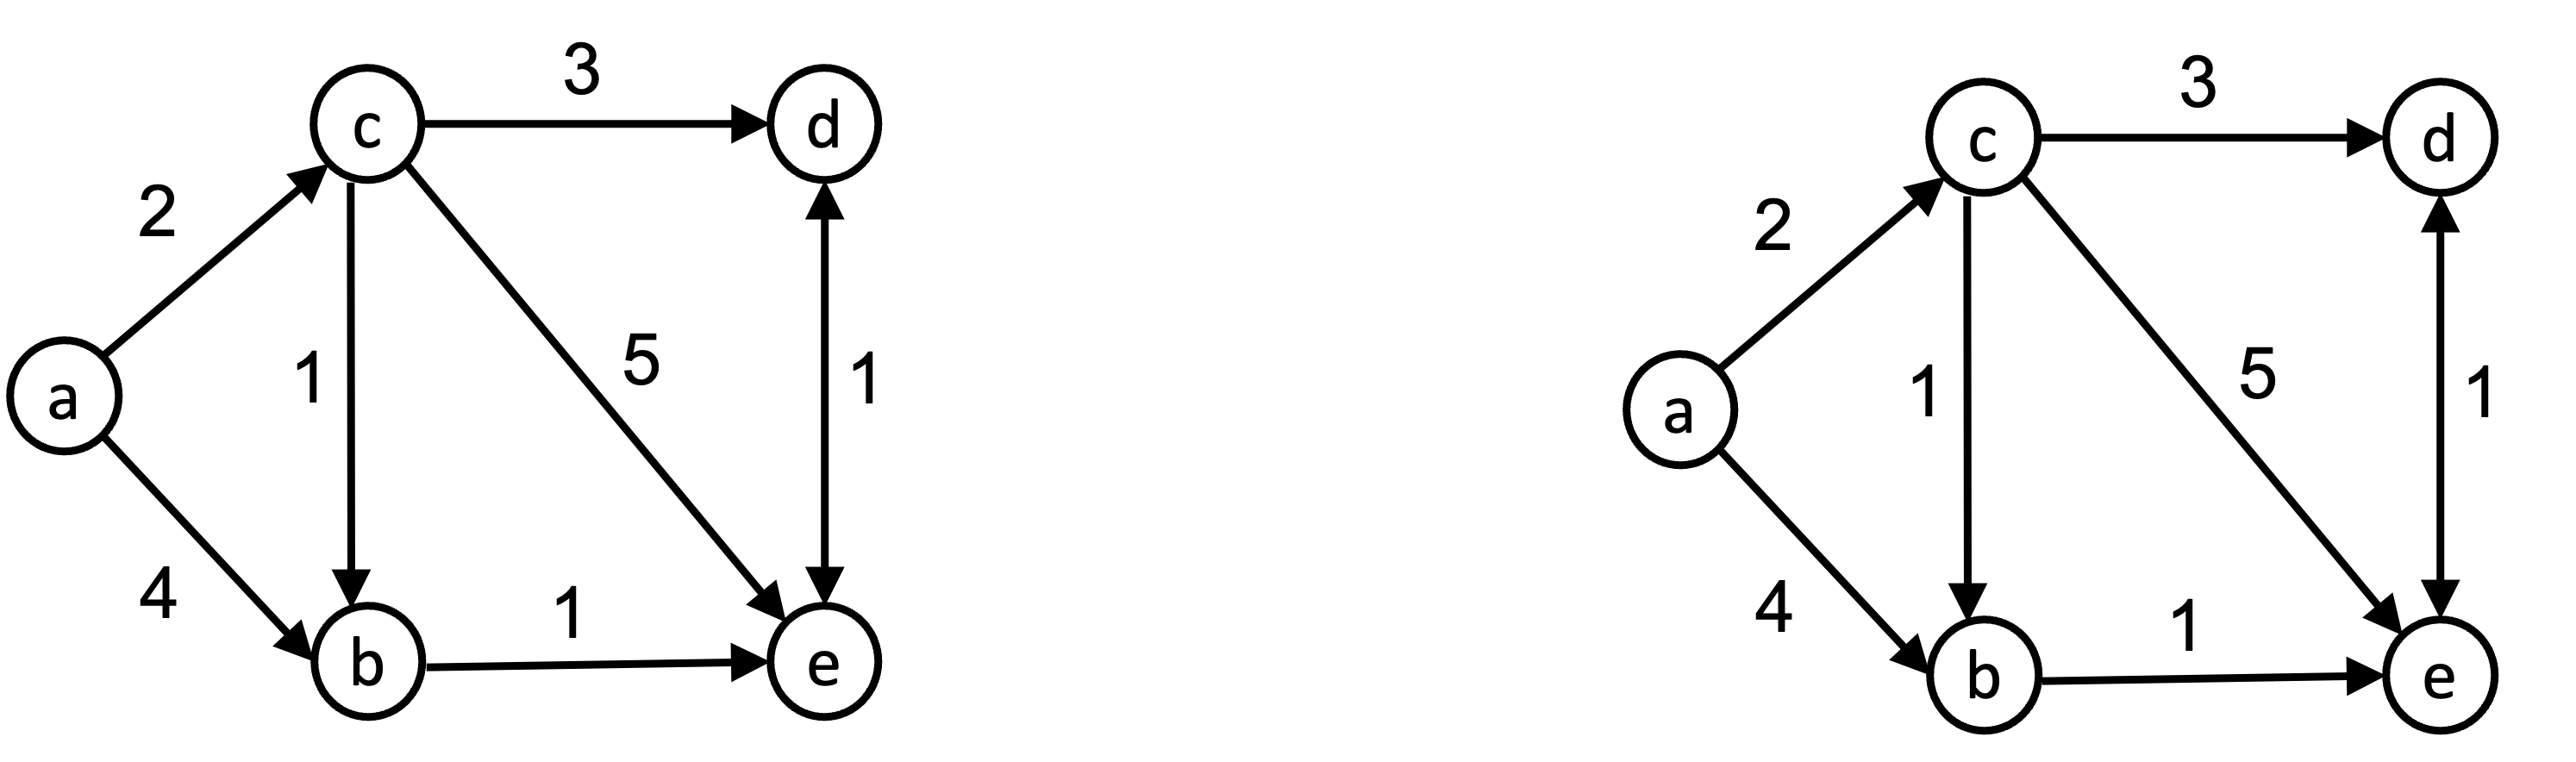
\includegraphics[width = \linewidth]{twographs.png}
	
	\newpage
	
	\subsection{Correctness}
	\begin{theorem}
		Assuming that $G = (V,E,w)$ has no negative edges, when \textsc{Bellman-Ford} terminates, $v.d$ will equal $\delta(s,v)$ for every $v \in V$. 
	\end{theorem}
	
	
	\newpage
	
	
	\subsection{Catching Negative Cycles}
	\begin{algorithm}
		\textsc{Bellman-Ford} (Negative cycle check)
		\begin{algorithmic}
			\State Do everything else...
			\For{$ (u,v) \in E$}
			\If{$v.d > u.d + w(u,v)$}
			\State Return an error, the graph has a negative cycle
			\EndIf
			\EndFor
		\end{algorithmic}
	\end{algorithm}
	
	\begin{theorem}
		If $G = (V,E,w)$ has a negative weight cycle that is reachable from $s$, then the code above will produce an error
	\end{theorem}
	
	\newpage
	
		\section{Dijkstra's Algorithm}
	\begin{algorithm}
		\textsc{Dijkstra}$(G,w,s)$
		\begin{algorithmic}
			\State \textsc{Initialize-SSSP}$(G,w,s)$
			\State $S = \emptyset$
			\State $Q = V$
			\While{$Q \neq \emptyset$}
			\State $u = \textsc{ExtractMin}(Q)$
			\State $S = S \cup \{u\}$
			\For{$v \in \text{Adj}[u]$}
			\State \textsc{Relax}($u,v,w$)
			\EndFor
			\EndWhile
		\end{algorithmic}
	\end{algorithm}
	
	This algorithm maintains:
	\begin{itemize}
		\item $S$ = set of vertices for which $v.d = \delta(s,d)$
		\item $Q$ = min-priority queue storing $v.d$ for all vertices in $V-S$ 
	\end{itemize}
	\vs{2cm}
	\begin{Qu}
		How many times does the while loop in Dijkstra's algorithm iterate?
		\begin{itemize}
			\aitem $O(V)$ times
			\bitem $O(E)$ times
			\citem $O(EV)$ times
			\ditem Depends on the graph
		\end{itemize}
	\end{Qu}
	
	
	\newpage
	
	\subsection{Example}
	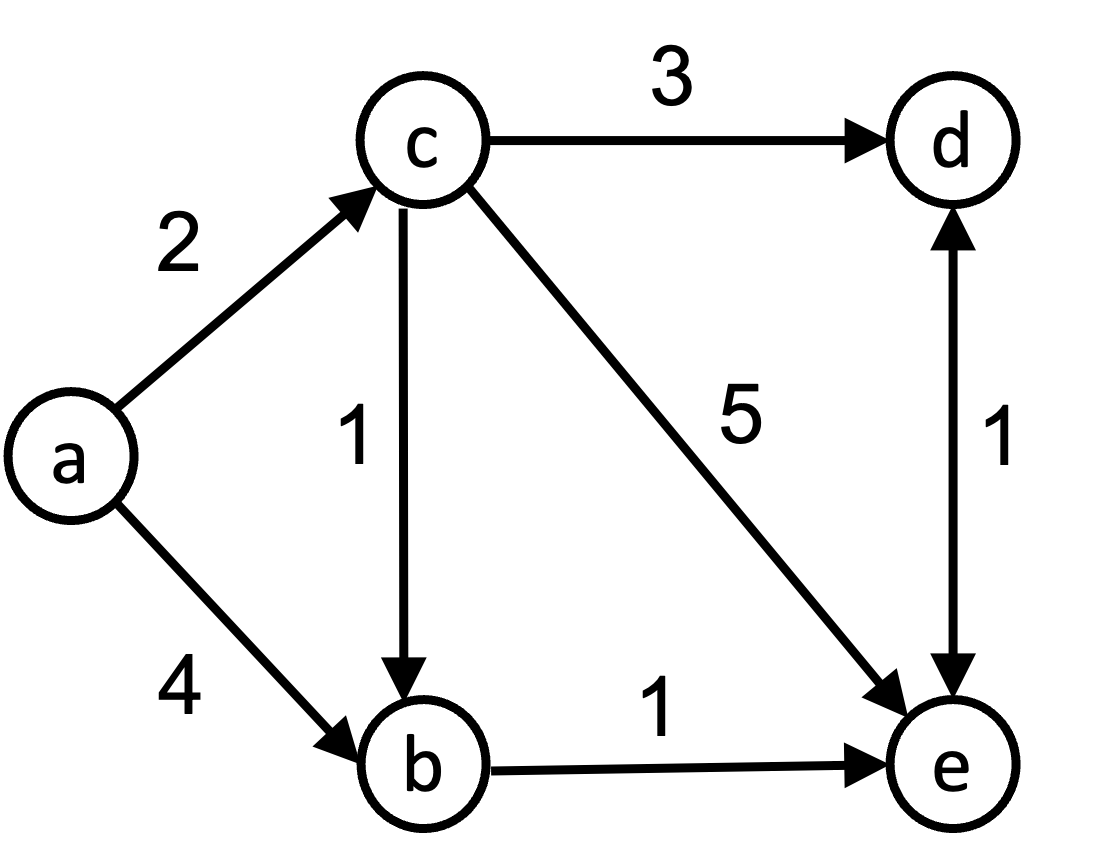
\includegraphics[width = .45\linewidth]{small-graph-sssp.png}
	
	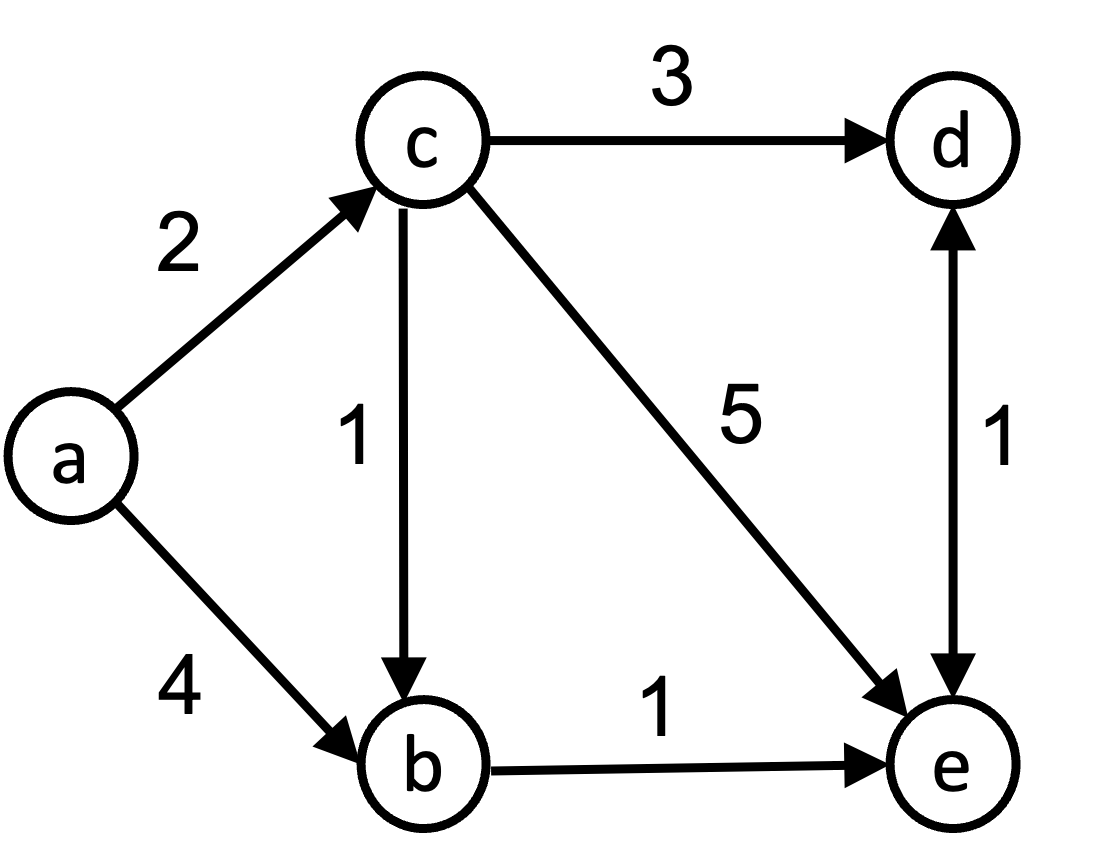
\includegraphics[width = .45\linewidth]{small-graph-sssp.png}
	
	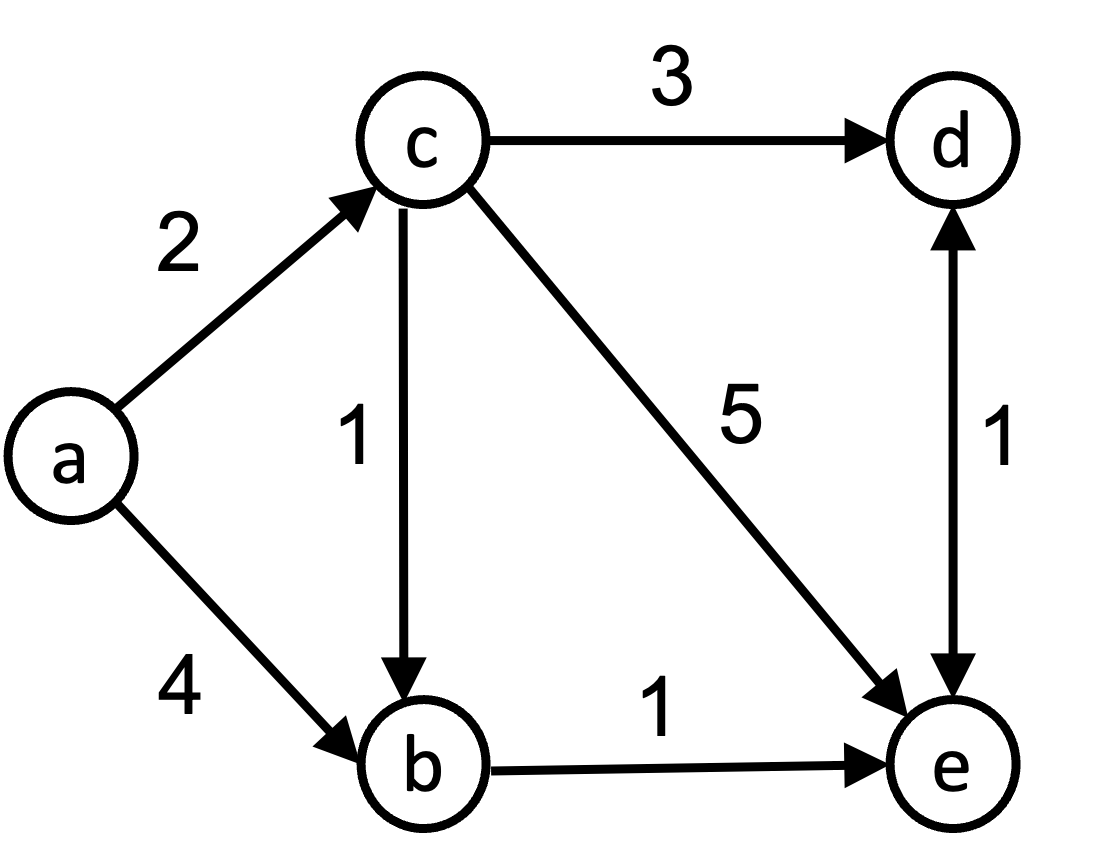
\includegraphics[width = .45\linewidth]{small-graph-sssp.png}
	
	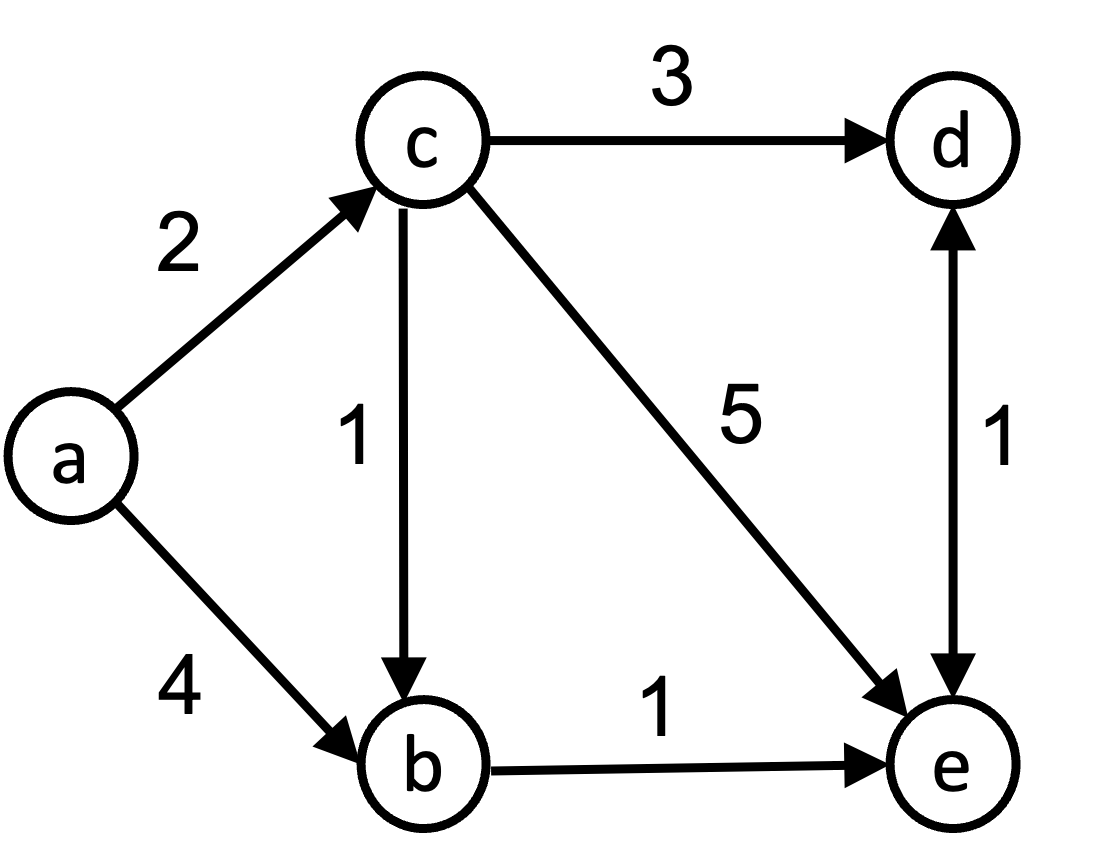
\includegraphics[width = .45\linewidth]{small-graph-sssp.png}
	\newpage
	\subsection{Correctness}
	\vspace{-20pt}
	\begin{algorithm}
		\textsc{Dijkstra}$(G,w,s)$
		\begin{algorithmic}
			\State \textsc{Initialize-SSSP}$(G,w,s)$
			\State $S = \emptyset$
			\State $Q = V$
			\While{$Q \neq \emptyset$}
			\State $u = \textsc{ExtractMin}(Q)$
			\State $S = S \cup \{u\}$
			\For{$v \in \text{Adj}[u]$}
			\State \textsc{Relax}($u,v,w$)
			\EndFor
			\EndWhile
		\end{algorithmic}
	\end{algorithm}
	We will take the following properties as given.
	
	\paragraph{Upper bound property}
	For each $v \in V$, the property $v.d \geq \delta(s,v)$ is maintained throughout the algorithm.\\
	
	\paragraph{Convergence property}
	Let $p = \{s, \hdots , u,v\}$ be a shortest path involving an edge $(u,v) \in E$. If $u.d = \delta(s,u)$ at any time prior to relaxing edge $(u,v)$, then $v.d = \delta(s,v)$ after relaxing $(u,v)$.\\
	
	\paragraph{No path property}
	If there is no path from $s$ to $v$, then $v.d = \delta(s,v) = \infty$ throughout the algorithm. \\ \\
	
	
	\begin{theorem}
		Dijkstra's algorithm, run on a weighted, directed graph $G = (V,E,w)$ with positive weights and source $s \in V$, terminates with $u.d = \delta(s,u)$ for all $u \in V$
	\end{theorem}
	\textit{Proof.} We maintain the following invariant throughout. \\
	
	\textbf{Invariant}: At the start of the while loop, the node $u$ added to $S$ satisfies $u.d = \delta(s,u)$. \\
	
	If this invariant is true, the theorem is shown. Why?
	\newpage
	
	Assume this invariant is \emph{not} true and we will show a contradiction. \\
	
	Define $u$ to be the first node added to $S$ where $u.d \neq \delta(s,u)$.
	
	\begin{enumerate}
		\item We know $u \neq s$. \\
		\item We know there is a path from $s$ to $u$. \\
		\item Let $p$ be a shortest path from $s$ to $u$, which goes from $S$ to $V-S$, let $y$ be the first node in $p$ from $V-S$ in this path, and $x$ be its predecessor. \\ 
		\vs{4cm} 
		\item We know $x.d = \delta(s,x)$\\
		\item We then know $y.d = \delta(s,y)$ \\
		\item We know that $\delta(s,y) \leq \delta(s,u)$ \\
		
		\item And we know $\delta(s,u) \leq u.d$ \\
		\item We know also that $u.d \leq y.d$ \\
		\item The last steps show $y.d = \delta(s,y) \leq \delta(s,u) \leq u.d \leq y.d$. Why is this a contradiction?
	\end{enumerate}
	
	\newpage
	
	
	\subsection{Runtime Analysis}
	\begin{algorithmic}
		\State \textsc{Initialize-SSSP}$(G,w,s)$
		\State $S = \emptyset$; $Q = V$
		\While{$Q \neq \emptyset$}
		\State $u = \textsc{ExtractMin}(Q)$
		\State $S = S \cup \{u\}$
		\For{$v \in \text{Adj}[u]$}
		\If{$v.d > u.d + w(u,v)$}
		\State $v.d = u.d + w(u,v)$
		\State $v.\pi = u$
		\EndIf
		\EndFor
		\EndWhile
	\end{algorithmic}
	\begin{Qu}
		Assuming that all nodes are reachable from $s$, what runtime we can obtain for Dijkstra's algorithm? (Warning: there may be more answer that you can argue is valid! Don't just select an answer, think about a specific reasoning for the runtime analysis you select).
		\begin{itemize}
			\aitem $O(V + E)$ 
			\bitem $O(V^2)$
			\citem $O(VE)$
			\ditem $O(E \log V)$
			\eitem $O(E + V \log V)$
		\end{itemize}
	\end{Qu}
	
	
	\newpage
	\subsection{Class Activity: another example}
	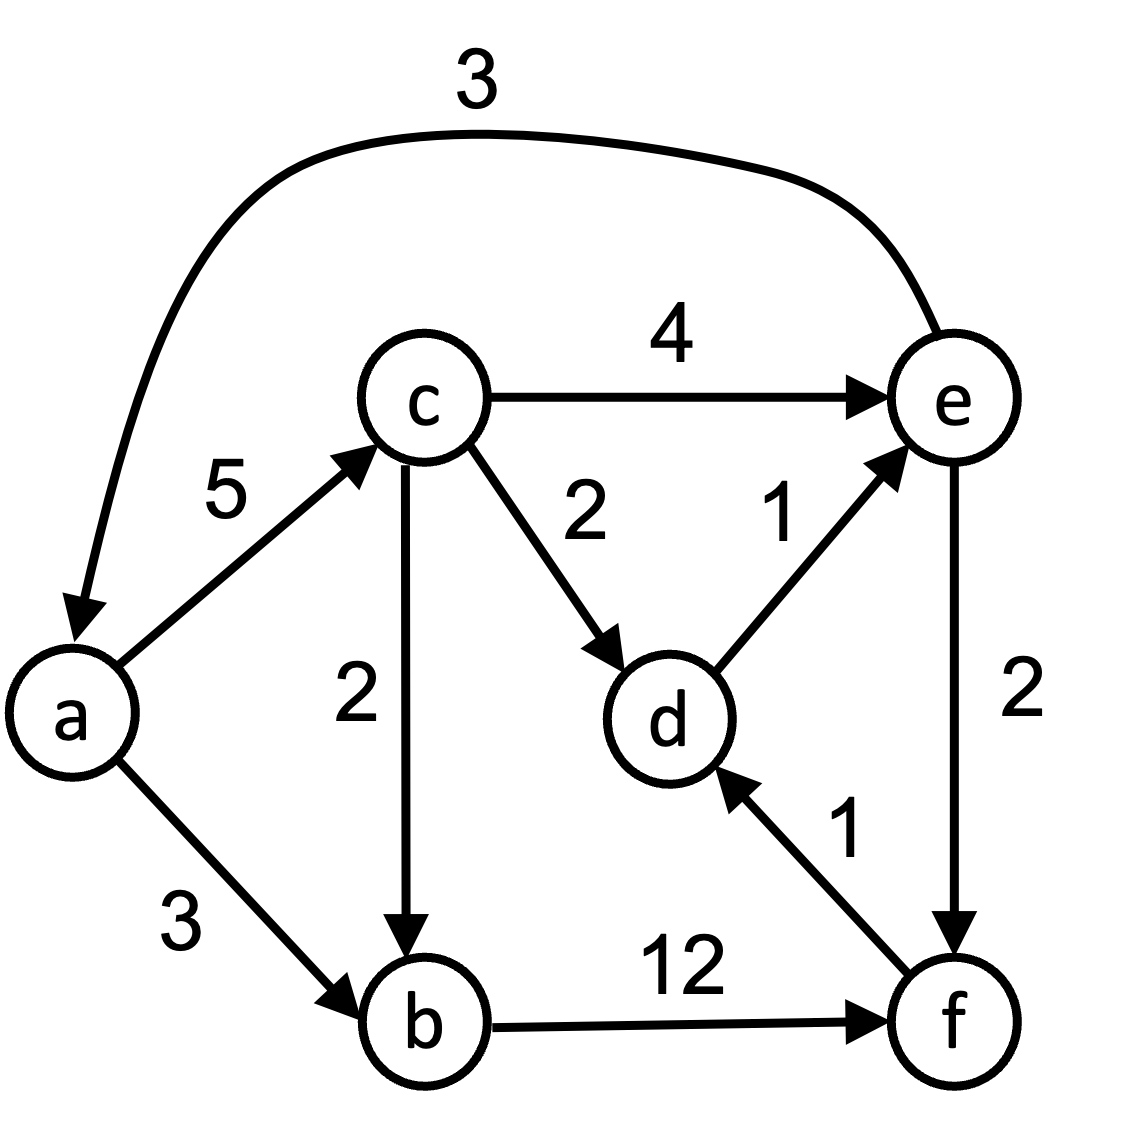
\includegraphics[width = .75\linewidth]{dijkstrasalg.png}
	
\end{document}